\documentclass[aspectratio=169,11pt]{beamer}
\usepackage{fontspec,xeCJK}
\setmainfont{texgyreheros-regular.otf}[BoldFont=texgyreheros-bold.otf,ItalicFont=texgyreheros-italic.otf]
\setsansfont{texgyreheros-regular.otf}[BoldFont=texgyreheros-bold.otf,ItalicFont=texgyreheros-italic.otf]
\setCJKmainfont{HaranoAjiGothic-Regular.otf}[BoldFont=HaranoAjiGothic-Bold.otf]
\setCJKsansfont{HaranoAjiGothic-Regular.otf}[BoldFont=HaranoAjiGothic-Bold.otf]
\usepackage{amsmath,amssymb,booktabs,array,tikz}
\usetikzlibrary{arrows.meta,patterns,decorations.markings}
\definecolor{ink}{HTML}{17324D}
\definecolor{accent}{HTML}{157C85}
\definecolor{light}{HTML}{EFF5F6}
\definecolor{muted}{HTML}{536575}
\setbeamercolor{normal text}{fg=ink,bg=white}
\setbeamercolor{frametitle}{fg=ink,bg=white}
\setbeamercolor{structure}{fg=accent}
\setbeamercolor{block title}{fg=white,bg=accent}
\setbeamercolor{block body}{fg=ink,bg=light}
\setbeamerfont{frametitle}{size=\Large,series=\bfseries}
\setbeamersize{text margin left=8mm,text margin right=8mm}
\setbeamertemplate{navigation symbols}{}
\setbeamertemplate{frametitle}{\vspace{2mm}\insertframetitle\par\vspace{1.5mm}{\color{accent}\hrule height .6pt}}
\setbeamertemplate{footline}{\hspace{8mm}\color{muted}\fontsize{6}{7}\selectfont Zenstudy\quad 熱力学\hfill\insertframenumber\hspace{8mm}\vspace{2mm}}
\setlength{\parskip}{3pt}
\newcommand{\tagline}[1]{{\small\color{accent}\textbf{#1}}\par\vspace{1mm}}
\newcommand{\ask}[2]{\par\vspace{2mm}\textcolor{accent}{\textbf{(#1)}}\quad #2\par}
\newcommand{\baseeq}{pV=nRT,\qquad U=\frac32nRT,\qquad Q=\Delta U+W}
\newcommand{\cyclefig}{%
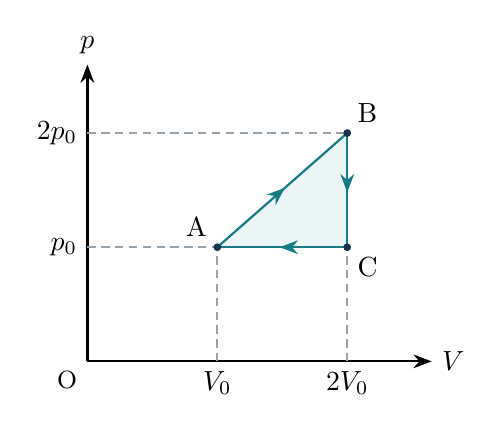
\begin{tikzpicture}[x=1.65cm,y=1.45cm,>=Stealth,line width=.8pt]
\fill[accent!8] (1,1)--(2,2)--(2,1)--cycle;
\draw[->] (0,0)--(2.65,0) node[right]{$V$};
\draw[->] (0,0)--(0,2.6) node[above]{$p$};
\node[below left] at (0,0) {\small O};
\draw[densely dashed,muted!60] (0,1)--(1,1) (0,2)--(2,2) (1,0)--(1,1) (2,0)--(2,1);
\node[left] at (0,1) {$p_0$}; \node[left] at (0,2) {$2p_0$};
\node[below] at (1,0) {$V_0$}; \node[below] at (2,0) {$2V_0$};
\draw[accent,thick,postaction={decorate},decoration={markings,mark=at position .52 with {\arrow{Stealth}}}] (1,1)--(2,2);
\draw[accent,thick,postaction={decorate},decoration={markings,mark=at position .52 with {\arrow{Stealth}}}] (2,2)--(2,1);
\draw[accent,thick,postaction={decorate},decoration={markings,mark=at position .52 with {\arrow{Stealth}}}] (2,1)--(1,1);
\foreach \x/\y in {1/1,2/2,2/1}{\fill[ink] (\x,\y) circle(1.4pt);}
\node[above left] at (1,1) {A}; \node[above right] at (2,2) {B}; \node[below right] at (2,1) {C};
\end{tikzpicture}}
\newcommand{\pistonfig}{%
\begin{tikzpicture}[x=.82cm,y=.82cm,>=Stealth,line width=.8pt]
\fill[accent!8] (.25,.25) rectangle(3.3,2.55);
\fill[pattern=north east lines,pattern color=muted!50] (0,0) rectangle(.25,2.8);
\fill[pattern=north east lines,pattern color=muted!50] (0,2.55) rectangle(4.8,2.8);
\fill[pattern=north east lines,pattern color=muted!50] (0,0) rectangle(4.8,.25);
\draw[thick] (4.8,0)--(0,0)--(0,2.8)--(4.8,2.8);
\draw[thick] (4.8,.25)--(.25,.25)--(.25,2.55)--(4.8,2.55);
\filldraw[fill=muted!25,thick] (3.3,.25) rectangle(3.58,2.55);
\draw[very thick,<-] (3.58,1.4)--(5.4,1.4) node[right]{$F$};
\node at (1.7,1.65) {理想気体};
\node at (1.7,1.05) {$p,\ V,\ T$};
\node[font=\small] at (4.45,2.1) {真空};
\draw[fill=white,line width=1.4pt,accent] (1.05,.08)--(2.1,.08);
\draw[accent,->] (1.55,-.65)--(1.55,.0);
\node[below,font=\small] at (1.55,-.65) {熱窓（開閉式）};
\draw[muted] (3.45,2.58)--(3.45,3.15);
\node[above,font=\small] at (3.45,3.15) {ピストン・断面積 $S$};
\end{tikzpicture}}
